\section{Mise en pratique}

Le premier résultat que nous aimerions obtenir est le calcul du groupe fondamental du cercle. Nous verrons que celui-ci est isomorphe à $\bb{Z}$, puisque cela revient à compter le nombre de tour qu'un lacet fait autour du cercle.

Intuitivement, nous devons comprendre que le lacet faisant une fois le tour du cercle (disons le lacet $t\mapsto e^{2i\pi t}$) ne peut se rétracter en le lacet constant. Cela vient du fait que l'on ne peut pas couper le lacet, ni passer au travers le trou à l'intérieur du cercle.

\subsection{Revêtements, première partie}\label{covering-space-intro}

\begin{wrapfigure}{r}{0.2\textwidth}
    \centering
    \includegraphics[width=.9\linewidth]{pictures/covering-map-circle.png}
    \caption{\centering Revêtement du cercle}
    \label{fig:cover-circle}
\end{wrapfigure}

Pour comprendre ce qu'est qu'un \emph{revêtement}, nous allons commencer par un exemple classique, celui du cercle.

\begin{exemple}
Nous nous plaçons dans l'espace euclidien en trois dimensions. Notre cercle, ici appelé $X$, se retrouve en dessous d'un autre espace, qui est appelé ici $Y$. La projection $p$ projette $Y$ sur le cercle, ne dépendant pas de la troisième coordonnée.

Le revêtement du cercle $X$ est ici le couple $(Y,p)$. Ce que l'on peut voir sur la figure, est que la préimage ouverte de l'ouvert $U\subset X$ par $p$ est une réunion disjointe d'ouvert $(S_i)_i\subset Y$. On note alors $p\inv=\sqcup_i S_i$. De plus, la projection restreinte à un ouvert $S_i\in p\inv(U)$ nous donne un homéomorphisme avec $U$. Autrement dit, nous avons la projection $p|_{S_i}:S_i\to U$ qui est un homéomorphisme, dit local.

Nous pouvons définir ce revêtement de deux manières différentes. La première est de considérer $Y=\{\big(\cos(2\pi t),\sin(2\pi t), t\big),t\in \bb{R}\}$, et la projection définie simplement par $p:(x,y,z)\in Y\mapsto(x,y)\in X$. La deuxième manière est de remarquer que l'hélice est homéomorphe à $\bb{R}$ (en la déroulant sur l'axe des abscisses) : nous pouvons alors simplifier et dire que $Y=\bb{R}$, et définir la projection $p:t\mapsto\big(\cos(2\pi t),\sin(2\pi t)\big)$ sur le cercle.
\end{exemple}

\begin{definition}
Un \emph{revêtement} d'un espace $X$ est un espace $\Tilde{X}$ ainsi qu'une projection $p:\Tilde{X}\to X$, tels que : il existe un recouvrement ouvert $\{U_i\}_{i\in I}$ de $X$, de telle sorte que pour chaque $i\in I$,  $p\inv(U_i)$ est une union disjointe d'ouvert $V_{ij}$ de $\Tilde{X}$. Pour chaque $V_{ij}$, la projection restreinte $p|_{V_ij}:V_{ij}\to U_i$ induit un homéomorphisme.
\end{definition}

On parle dans ce cas d'\emph{homéomorphisme local}, lorsque l'application suffisamment restreinte tel que dans la définition induit un homéomorphisme.

\bigskip Cet espace possède de bonnes propriétés, tel que la \emph{propriété de relèvement de chemin} et la \emph{propriété de relèvement d'homotopie}, que nous énonçons juste après. Ces propriétés sont omniprésentes pour les calculs de groupes fondamentaux, comme celui du cercle.

Pour les propositions qui suivent, nous supposons que l'espace $X$ admet un revêtement.

\begin{proposition}\label{prop:rel-path}
Soit $X$ un espace et soit $(\Tilde{X},p)$ un revêtement de $X$. Pour un chemin $\gamma$ dans~$X$ partant de $x_0\in X$, en chaque point $\Tilde{x}_0\in p\inv(x_0)$, il existe un unique \emph{relèvement} $\Tilde{\gamma}:[0,1]\to\Tilde{X}$ partant de $\Tilde{x}_0$, ie. tel que $\gamma=p\Tilde{\gamma}$.
\end{proposition}

Ensuite vient la propriété de relèvement d'homotopie.

\begin{proposition}\label{prop:rel-hom}
Soit $X$ un espace et soit $(\Tilde{X},p)$ un revêtement de $X$. Pour une homotopie $\gamma_t$ de chemins de $X$ partant de $x_0$, en chaque point $\Tilde{x}_0~\in p\inv(x_0)$, il existe un unique relèvement d'homotopie $\Tilde{\gamma}_t:[0,1]\to\Tilde{X}$ commençant en $\Tilde{x_0}$, ie. tel que~$\gamma_t=p\Tilde{\gamma}_t$, pour tout $t\in[0,1]$.
\end{proposition}

En réalité, ces deux propositions proviennent d'un résultat encore plus général, mais qui peut paraître plus abstrait. Néanmoins, bien que la preuve reste elle aussi abstraite et se traite dans un sens topologique, elle reste intuitive et logique, et se déroule plutôt bien.

Voici donc le résultat général.

\begin{theorem}
Soit $X$ un espace et soit $(\Tilde{X},p)$ un revêtement de $X$. Étant donné une application~$F:Y\times[0,1]\to X$, et une application $\Tilde{F}_0:Y\times\{0\}\to\Tilde{X}$ relevant~$F|_{Y\times\{0\}}$, alors il existe une unique application $\Tilde{F}$ relevant $F$, et qui coïncide avec $\Tilde{F}_0$ sur $Y\times\{0\}$.
\end{theorem}
Nous pouvons d'ores et déjà voir que cette propriété est un cas général des deux autres. Si l'on prend $Y$ un singleton, alors nous avons la propriété de relèvement de chemin, tandis que si $Y=[0,1]$, alors nous avons la propriété de relèvement d'homotopie.

\begin{proof}
Supposons qu'il existe un recouvrement ouvert~$(U_i)_{i\in I}$ tel que l'on puisse définir un revêtement $\Tilde{X}$ de $X$. En reprenant les notations de l'énoncé, la continuité de $F$ implique que pour chaque $(y_0,t)\in Y\times[0,1]$, il existe un voisinage $V_t\times[a_t,b_t]$ de $(y_0,t)$ tel que $F(V_t\times[a_t,b_t])\subset U_l$ pour un certain $l$ dans $I$.

Soit $y_0\in Y$. La compacité de $\{y_0\}\times[0,1]$ implique l'existence d'un recouvrement ouvert $V_t\times[a_t,b_t]$ fini. Dans ce cas, nous pouvons nous intéresser à un voisinage $V\in\mathcal{V}(y_0)$\textbf{[qui est V ?]}, et à une partition de [0,1], que l'on note $$0=t_0<\cdots<t_m=1,$$de telle sorte que  pour tout $i\in\{0,..., m-1\}$, il existe $l\in I$ tel que l'on ait~$F(V\times[t_i,t_{i+1}])\subset U_l$, que l'on notera $U_i$.

\bigskip Par récurrence, supposons que l'application $\Tilde{F}$ ait été définie sur $V\times[0,t_i]$. Par définition du revêtement, nous savons qu'il existe un ouvert $\Tilde{U}_i\subset\bb{R}$ tel que la projection $p:\Tilde{U}_i\to U_i$ soit un homéomorphisme, vérifiant $\Tilde{F}(y_0,t_i)\in\Tilde{U}_i$. En notant l'intersection~$O=(V\times\{t_i\})\cap\Tilde{F}|_{V\times\{t_i\}}\inv(\Tilde{U}_i)$, on obtient alors $\Tilde{F}(O)\subset\Tilde{U}_i$. Dès lors, on peut définir $\Tilde{F}$ sur $[t_i,t_{i+1}]$ par la composition $p\inv F$.

\bigskip En remarquant que l'initialisation est supposée dans l'énoncé, nous pouvons ainsi construire $\Tilde{F}$ sur $V\times[0,1]$. Pour montrer que l'on peut le construire sur tout $Y$ en réitérant le procédé, nous devons d'abord montrer l'unicité de $\Tilde{F}$. Pour cette partie, nous considérerons l'ensemble $\{y_0\}\times[0,1]$ avec~$y_0\in Y$, dont nous nous permettons d'omettre le singleton, afin d'alléger les notations, puisqu'il n'impacte pas le raisonnement qui suit.

\bigskip Supposons $\Tilde{F}$ et $\Tilde{F}'$ deux relèvements de $F:[0,1]\to X$ tels que $\Tilde{F}(0)=\Tilde{F}'(0)$. Comme précédemment, on sait qu'il existe une partition $0=t_0<\cdots<t_m=1$ telle que chaque intervalle $[t_i,t_{i+1}]$ soit contenu dans un certain $U_i$.

Par récurrence, supposons que $\Tilde{F}([0,t_i])=\Tilde{F}'([0,t_i])$. Comme $[t_i,t_{i+1}]$ est un intervalle connexe, alors par continuité on sait que $\Tilde{F}'([t_i,t_{i+1}])$ est inclus dans un seul $\Tilde{U}_i$ tel que $p:\Tilde{U}_i\to U_i$ est un homéomorphisme.

Nous avons en particulier $\Tilde{F}(t_i)=\Tilde{F}'(t_i)$. Par injectivité de $p|_{\Tilde{U}_i}$, et du fait que $p\Tilde{F}=p\Tilde{F}'$, on sait également que $\Tilde{F}([t_i,t_{i+1}])\subset\Tilde{U}_i$. Toujours par injectivité de $p$, nous en déduisons donc que~$\Tilde{F}([t_i,t_{i+1}])=\Tilde{F}'([t_i,t_{i+1}])$.

\bigskip Finalement, on obtient par récurrence que $\Tilde{F}=\Tilde{F}'$ sur [0,1]. Ainsi, par unicité du revêtement sur $\{y_0\}\times[0,1]$, on peut alors construire une application $\Tilde{F}$ sur chaque ouvert $V\times[0,1]$ de manière unique, de telle sorte que chaque chevauchement d'ouvert définisse la même application. Cela veut alors dire que l'on peut définir correctement l'application $\Tilde{F}$ sur $Y\times[0,1]$. Étant une application continue sur chaque $V\times[0,1]$, $\Tilde{F}$ est continue sur $Y\times[0,1]$.
\end{proof}

Désormais, nous avons toutes les cartes en main pour pouvoir calculer le groupe fondamental du cercle.

\subsection{Le groupe fondamental du cercle}

\begin{wrapfigure}{l}{0.3\textwidth}
    \centering
    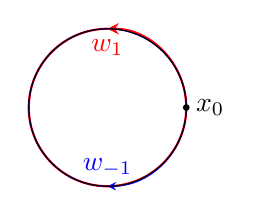
\begin{tikzpicture}
    \draw[thick, ->, red, >=stealth] (0, 1) arc[start angle=90, end angle=450, radius=1] node[below] {$w_1$};
    \draw[, ->, blue, >=stealth] (0, -1) arc[start angle=-90, end angle=-450, radius=1] node[above] {$w_{-1}$};
    % cercle centré
    \draw[black] (0,0) circle (1cm);
    \filldraw[black] (1,0) circle (1pt) node[right] {$x_0$};
    \end{tikzpicture}
    \caption{}
    \label{fig:loops-circle}
\end{wrapfigure}

Comme je le disais en introduction de cette section, les lacets dans le cercle sont définis par rapport à leur nombre de tours. C'est donc dans cette optique que nous allons utiliser une notation de lacets dépendant de celui-ci.

Nous définissons le lacet $w_n:s\in[0,1]\mapsto e^{2in\pi s}$ basé en $(1,0)$, faisant $n\in\bb{Z}$ tours autour du cercle de manière linéaire. Comme nous le montre la figure \ref{fig:loops-circle}, le sens considéré est trigonométrique, ou inverse des aiguilles d'une montre.

\begin{theorem}\label{th:grp-funda-circle}
L'application $\Phi:\bb{Z}\to\pi_1(\s{1})$, qui à un entier $n$ renvoie la classe d'homotopie $[w_n]$, est un isomorphisme.
\end{theorem}

\begin{proof}
Pour la démonstration, nous considérons le revêtement du cercle ${p:t\in\bb{R}\mapsto e^{2i\pi t}}$. En définissant le chemin $\Tilde{w}_n:s\in[0,1]\mapsto ns$, allant de 0 vers~$n\in\bb{Z}$, nous avons $p\Tilde{w}_n=w_n$. Cela veut ainsi dire que l'on peut redéfinir $\Phi$ comme étant une application qui envoie $n$ vers la classe d'homotopie du lacet $p\Tilde{\gamma}$, pour~$\Tilde{\gamma}$ un chemin allant de $0$ vers $n$. Sur $\bb{R}$, nous pouvons définir l'homotopie linéaire entre~$\Tilde{\gamma}$ et $\Tilde{w}_n$, puisque leurs extrémités coïncident. Par l'unicité du relèvement de lacets, nous pouvons ainsi en déduire $p\Tilde{\gamma}\simeq p\Tilde{w}_n=w_n$. Cela nous permet donc de définir différemment $\Phi$.

\bigskip Pour montrer que l'application $\Phi$ définit un morphisme, il suffit de montrer que pour $n$ et~$m$ deux entiers, nous avons $[\tilde{w}_n][\tilde{w}_m]=[\tilde{w}_{n+m}]$, c'est à dire que l'on a~$\tilde{w}_n\cdot \tilde{w}_m\simeq \tilde{w}_{n+m}$. En définissant la translation $\tau_m:x\mapsto x+m$, nous pouvons dire que $\Tilde{w}_n\cdot(\tau_n \tilde{w}_m)=w_{n+m}$, tandis que~$p\big(\Tilde{w}_n\cdot(\tau_n \Tilde{w}_m)\big)=w_n\cdot w_m$ et~$p(\Tilde{w}_{n+m})=w_{n+m}$.

Pour montrer que nous avons un isomorphisme, nous allons utiliser les deux propositions \ref{prop:rel-path} et \ref{prop:rel-hom}. En ce qui concerne la surjectivité, on considère un lacet $\gamma$ basé en $x_0=(1,0)$, représentant de $\alpha\in\pi_1(\s{1},x_0)$. Par la propriété de relèvement de chemin, il existe un chemin $\Tilde{\gamma}$ partant de 0, et finissant en un certain $n\in\bb{Z}$, car $p\Tilde{f}(1)=x_0$ et $p\inv(x_0)=\bb{Z}$. Par la redéfinition effectué au début de la démonstration, nous avons $\Phi(n)=[p\Tilde{\gamma}]=[\gamma]$.

Pour montrer que $\Phi$ est injective, supposons $\Phi(n)=\Phi(m)$, autrement dit que l'on a $w_n\simeq w_m$, avec $\gamma_t$ l'homotopie associée. Par la propriété de relèvement d'homotopie, nous savons qu'il existe une homotopie de chemin $\Tilde{\gamma}_t$ partant de 0. L'unicité de la propriété nous permet de dire que l'on a~$\Tilde{\gamma}_0=\Tilde{w}_n$ ainsi que~$\Tilde{\gamma}_1=\Tilde{w}_m$. Puisque l'homotopie ne change pas les extrémités, c'est à dire~$\Tilde{\gamma}_t(1)$ est fixe pour tout $t\in[0,1]$, nous avons $n=\Tilde{\gamma}_0(1)=\Tilde{\gamma}_1(1)=m$.

\bigskip Nous pouvons ainsi en conclure que $\Phi$ définit un isomorphisme entre le groupe fondamental du cercle et $\bb{Z}$.
\end{proof}

Ce résultat possède quelques utilisations directe, tel que le théorème de Brouwer en dimension~2 (voir \textbf{[ref Brouwer]}, ou encore le théorème fondamental de l'algèbre (voir th1.8 \textbf{[ref allen hatcher]}). Nous allons ici plutôt voir un résultat permettant le calcul de groupes fondamentaux d'autres espace, tel que le tore.

\begin{proposition}
Nous avons ${\pi_1(X\times Y)\cong\pi_1(X)\times\pi_1(Y)}$, pour tout couples d'espaces connexes par arc $X$ et $Y$.
\end{proposition}
\begin{proof}
Soit $\gamma$ un lacet de $X\times Y$. Il existe $\gamma_1$ et $\gamma_2$ lacets respectifs de $X$ et $Y$, tel que~${\gamma=(\gamma_1,\gamma_2)}$. De la même manière, on définit $\gamma'=(\gamma'_1,\gamma'_2)$ un lacet de $X\times Y$. Montrons que~${\gamma\simeq \gamma'}$ si et seulement si $\gamma_1\simeq\gamma'_1$ et $\gamma_2\simeq\gamma'_2$. Il suffit pour cela de voir que s'il existe une homotopie entre~$\gamma$ et $\gamma'$, alors il existe en particulier une homotopie entre $\gamma_1$ et $\gamma'_1$, ainsi qu'une homotopie entre $\gamma_2$ et~$\gamma'_2$. Et inversement, s'il existe une homotopie entre $\gamma_1$ et $\gamma'_1$, ainsi qu'une homotopie entre $\gamma_2$ et~$\gamma'_2$, l'homotopie produit est une homotopie entre $\gamma$ et $\gamma'$.

Nous pouvons alors définir une application $\Phi:[(\gamma_1,\gamma_2)]\mapsto([\gamma_1],[\gamma_2])$ pour tout $(\gamma_1,\gamma_2)$ lacets de~$X\times Y$. Cette application est un morphisme de groupe entre $\pi_1(X\times Y)$ et $\pi_1(X)\times\pi_1(Y)$, du fait que pour $[(\gamma_1,\gamma_2)],[(\gamma'_1,\gamma'_2)]\in\pi_1(X\times Y)$, nous avons : \[\begin{split}
\Phi([(\gamma_1,\gamma_2)][(\gamma'_1,\gamma'_2)])&=\Phi([(\gamma_1\cdot\gamma'_1,\gamma_2\cdot\gamma'_2)])\\
&=([\gamma_1\cdot\gamma'_1],[\gamma_2\cdot\gamma'_2])\\
&=([\gamma_1],[\gamma_2])([\gamma'_1],[\gamma'_2])\\
&=\Phi([\gamma_1],[\gamma_2])\Phi([\gamma_1],[\gamma_2]).
\end{split}\]Il s'agit d'un isomorphisme puisque l'application définit dans l'autre sens est également un morphisme.
\end{proof}

\begin{exemple}
Le tore en deux dimensions $T^2$ est défini comme étant le produit cartésien de deux cercles, on a $T^2=\s{1}\times\s{1}$. Une manière de se représenter ce fait est de voir le cercle comme l'intervalle $[0,1]$ sur lequel on recolle les extrémités~0 et 1. Ainsi, $\s{1}\times[0,1]$ forme un cylindre, et si l'on recolle les extrémités pour obtenir $\s{1}\times\s{1}$, nous formons le tore. Il s'agit de la méthode utilisée pour représenter le tore sous forme d'un polygone fondamental du tore.

\begin{figure}[H]
     \centering
     \includegraphics[width=0.5\linewidth]{pictures/TorusCircle_ManimCE_v0.18.1.png}
     \caption{Tore vu comme étant $\s{1}\times\s{1}$}
     \label{fig:torus-circle}
 \end{figure} 

La proposition nous permet de calculer le groupe fondamental du tore : \[\pi_1(T^2)=\pi_1(\s{1}\times\s{1})\cong\pi_1(\s{1})\times\pi_1(\s{1})\cong\bb{Z}^2\]Pour s'en persuader, il suffit de prendre deux générateurs : un lacet qui fait le tour de la "bouée", et un autre lacet qui fait le tour autour du trou. En notant $a$ le premier lacet et $b$ le second, on admet le fait qu'il existe une homotopie entre $ab$ et $ba$, qui intuitivement revient à décaler le moment où on effectue le tour de la bouée.

Nous pouvons généraliser ce calcul pour le tore à dimension $n>1$, définie comme étant $T^n=(\s{1})^n$. Son groupe fondamental est donc isomorphe à $\bb{Z}^n$.
\end{exemple}

Avec les outils que nous possédons dès à présent, il serait possible de calculer le groupe fondamental de la sphère de dimension quelconque. Nous allons plutôt voir un résultat plus fort, permettant de traiter ce cas de manière simple.

\subsection{Version faible du théorème de Van Kampen}

Si l'on peut décrire $X$ en tant que l'union de deux sous espaces $A$ et $B$, le théorème de Van Kampen stipule que l'on peut décrire son groupe fondamental en fonction de celui de $A$ et celui de $B$. Nous nous intéresserons à la version faible du théorème, c'est à dire lorsque $A\cap B$ forme un espace simplement connexe.

Mais avant de voir le théorème et ses applications, nous avons besoin d'introduire le produit libre de groupes.

\begin{definition}
Soient $G$ et $H$ deux groupes. Le \emph{produit libre} de $G$ et $H$, noté~$G\ast H$, est le l'ensemble des mots formé alternativement d'éléments de $G$ et d'éléments de $H$. On muni de la loi de concaténation, modulo les règles suivantes : \begin{itemize}
    \item Si une lettre est un élément neutre, alors elle est supprimée ;
    \item On a $(g)(g')=(gg')$ et $(h)(h')=(hh')$, pour tout $g,g'\in G$, et $h,h'\in H$.
\end{itemize}
Cela permet donc de former une loi de groupe sur cet ensemble $G\ast H$, avec l'élément neutre le mot vide, et l'inverse d'un mot comme étant le mot écrit à l'envers avec les inverses : $\Big((g_1)(h_1)\cdots(g_n)(h_n)\Big)\inv=(h_n\inv)(g_n\inv)\cdots(h_1\inv)(g_1\inv)$.
\end{definition}

\begin{exemple}
Soient $G=<g>$ et $H=<h>$. Les mots $ghg^2h^{-3}g^{12}, ghg^{-1}, hgh^2g^{-3}$ sont des exemples d'éléments appartenant au groupe $G\ast H$. L'inverse de $g^2h^3g^{-5}h$ est $h^{-1}g^5h^{-3}g^{-2}$.
\end{exemple}

\begin{theorem}[Van Kampen]\label{th:van-kampen}
Soit $X$ un espace, étant l'union de deux sous-espaces connexes par arc $A$ et $B$. Le morphisme $\pi_1(A)\ast\pi_1(B)\to\pi_1(X)$ est surjectif, et lorsque l'intersection $A\cap B$ est simplement connexe, il s'agit d'un isomorphisme.
\end{theorem}

L'idée est de décomposer les lacets de $X$ en des lacets de $A$ et des lacets de $B$. Le noyau du morphisme correspond au groupe fondamental de l'intersection, d'où le fait que l'on a un isomorphisme lorsque celui-ci est trivial. Pour une démonstration détaillé, le lecteur est invité à lire \href{https://www.normalesup.org/~fjacobe/Topo.pdf}{[TopoMa]}.

\subsubsection{Applications}
L'opérateur $\vee$, nommé \emph{bouquet} ou \emph{wedge sum} en anglais, sur les espaces permet de les joindre en un seul point. On obtient cet espace en effectuant le quotient de~$X\sqcup Y$ en identifiant deux points~$x_0\in X$ et~$y_0\in Y$.

\begin{exemple}
Le bouquet $\s{1}\vee\s{1}$, où l'on a identifié le point $(1,0)$ du premier cercle et le point $(-1,0)$ du second, nous donne une forme de $\infty$. Nous pouvons calculer son groupe fondamental grâce au théorème de Van Kampen.
\begin{figure}[H]
    \centering
    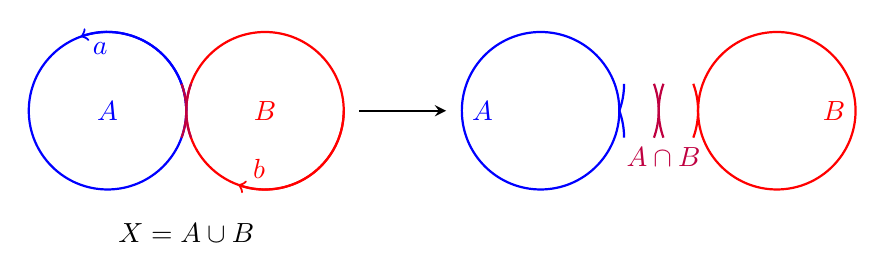
\begin{tikzpicture}
    \draw[thick, blue] (-1,0) circle (1cm) node{$A$};
    \draw[thick, red] (1,0) circle (1cm) node{$B$};
    \draw[thick, ->, blue] (0, 0) arc[start angle=0, end angle=110, radius=1]node[below left, near end]{$a$};
    \draw[thick, ->, red] (2, 0) arc[start angle=0, end angle=-110, radius=1]node[above left, near end]{$b$};
    \draw[thick, purple] (0,0) arc[start angle=0, end angle=-20, radius=1];
    \draw[thick, purple] (0,0) arc[start angle=0, end angle=20, radius=1];
    \draw[thick, purple] (0,0) arc[start angle=180, end angle=200, radius=1];
    \draw[thick, purple] (0,0) arc[start angle=180, end angle=160, radius=1];
    \draw[thick] (0,-1.3) arc[start angle=0, end angle=0, radius=1] node[below]{$X=A\cup B$};

    %A
    \draw[thick, blue] (5.5, 0) arc[start angle=0, end angle=360, radius=1]node[midway, right]{$A$};
    \draw[thick, blue] (5.5,0) arc[start angle=-20, end angle=0, radius=1];
    \draw[thick, blue] (5.5,0) arc[start angle=20, end angle=0, radius=1];
    %B
    \draw[thick, red] (6.5, 0) arc[start angle=180, end angle=-180, radius=1]node[midway, left]{$B$};
    \draw[thick, red] (6.5,0) arc[start angle=0, end angle=-20, radius=1];
    \draw[thick, red] (6.5,0) arc[start angle=0, end angle=20, radius=1];
    %AuB
    \draw[thick, purple] (6,0) arc[start angle=0, end angle=-20, radius=1];
    \draw[thick, purple] (6,0) arc[start angle=0, end angle=20, radius=1];
    \draw[thick, purple] (6,0) arc[start angle=180, end angle=200, radius=1] node[below] {$A\cap B$};
    \draw[thick, purple] (6,0) arc[start angle=180, end angle=160, radius=1];

    %arrow
    \draw[->, >=stealth, thick] (2.2,0) -- (3.3,0);
    \end{tikzpicture}
    \caption{Décomposition de $\s{1}\vee\s{1}$ pour le théorème de Van Kampen}
\end{figure}
Soit $X=\s{1}\vee\s{1}$, que nous décomposons comme sur la figure ci-dessus. Nous avons dans un premier temps les deux sous-espaces $A$ et $B$ homéomorphes au cercle. Leurs groupes fondamentaux sont donc également isomorphes à $\bb{Z}$. L'intersection $A\cap B$ est quant à elle simplement connexe, du fait qu'il s'agisse d'un point. Avec le théorème de Van Kampen, nous en déduisons le résultat suivant, en notant $x_0$ le point d'intersection des deux cercles : \[\pi_1(\s{1}\vee\s{1},x_0)\cong\pi_1(\s{1},(1,0))\ast\pi_1(\s{1},(-1,0))\cong\bb{Z}\ast\bb{Z}.\]En notant le lacet $a$ pour celui qui fait le tour du cercle bleu, et $b$ celui qui fait le tour du cercle rouge, nous avons bien deux générateurs libres du groupe. Il est important de remarquer ici que le groupe n'est pas abélien : il n'existe pas d'homotopie entre $ab$ et $ba$.
\end{exemple}

Nous pouvons alors calculer simplement le groupe fondamental de la sphère de dimension $n>1$.

\begin{proposition}
Pour $n>1$, la sphère $\s{n}$ est simplement connexe.
\end{proposition}
\begin{proof}
Montrons que le groupe fondamental de la sphère $\s{n}$ est trivial. Pour ce faire, nous considérons $A=\s{n}\setminus\{N\}$ et $B=\s{n}\setminus\{S\}$, avec $N$ et $S$ les points respectivement au nord et au sud de la sphère. Nous savons que $A$ et $B$ sont homéomorphes à $\bb{R}^n$, donc ces espaces sont simplement connexes.

Le théorème de Van Kampen, nous dit que le morphisme $0\ast0\to\pi_1(\s{n},x_0)$ est surjectif, ce qui nous permet de conclure que le groupe $\pi_1(\s{n},x_0)$ est trivial.
\end{proof}

La version forte du théorème est intéressante également, elle permet entre autres de calculer efficacement le groupe fondamental du plan projectif, avec un découpage astucieux (voir \href{https://www.math3ma.com/blog/the-fundamental-group-of-the-real-projective-plane}{[Math3ma]}). Pour ceux qui ne sont pas familier avec le plan projectif, je vous renvoie vers l'article \cite{Homeo-article} afin d'avoir une explication complète des différentes constructions. Voici tout de même une idée à avoir pour le calcul de son groupe fondamental.

\begin{exemple}
Initialement, le plan projectif réel $\bb{R}P^2$ désigne l'ensemble des droites vectorielles de~$\bb{R}^3$ passant par l'origine. Nous savons également qu'il peut être interprété comme le carré sur la figure~\ref{tkz:proj-plane}, et c'est cette représentation dont nous allons nous servir ici.


Notre objectif est d'avoir une représentation du groupe fondamental. Sur la figure \ref{tkz:proj-plane}, nous avons choisi comme point de base $x_0$ appartenant à la bordure. Comme il est identifié à son symétrique par rapport au centre du carré, il se trouve à la fois en haut à droite et à la fois en bas à gauche : c'est le même point ! Le chemin $\gamma$ traversant la diagonale désigne ainsi un exemple de lacet. Nous pouvons remarquer que nous ne pouvons pas rétracter ce lacet.

\begin{figure}[H]
\centering
\begin{subfigure}[t]{0.45\textwidth}
\centering
\begin{tikzpicture}[scale=.8]
    % fond gris
    \fill[gray!30] (0,0) rectangle (4,4);
    %flèche du haut
    \draw[thick, red, ->, >=stealth'] (0,4) -- (4,4) node[midway, below] {\textbf{A}};
    %flèche du bas
    \draw[thick, red, ->, >=stealth'] (4,0) -- (0,0) node[midway, above] {\textbf{A}};
    \draw[thick, blue, ->, >=stealth'] (0,0) -- (0,4) node[midway, right] {\textbf{B}};
    \draw[thick, blue, ->, >=stealth'] (4,4) -- (4,0) node[midway, left] {\textbf{B}};
    %carré
    \draw[black, line width=.0mm] (0,0) rectangle (4,4);
    
    %gamma
    \draw[thick, black, ->] (4,0) -- (2,2);
    \draw[thick, black] (2,2) -- (0,4) node[very near start, below]{$\gamma$};
    \filldraw[] (4,0) circle(1pt) node[right]{$x_0$};
    \filldraw[] (0,4) circle(1pt) node[left]{$x_0$};
\end{tikzpicture}
\caption{Le plan projectif et un lacet $\gamma$}
\label{tkz:proj-plane}
\end{subfigure}
\begin{subfigure}[t]{0.45\textwidth}
\centering
\begin{tikzpicture}[scale=.8]
    % fond gris
    \fill[gray!30] (0,0) rectangle (4,4);
    %flèche du haut
    \draw[thick, red, ->, >=stealth'] (0,4) -- (4,4) node[midway, below] {\textbf{A}};
    %flèche du bas
    \draw[thick, red, ->, >=stealth'] (4,0) -- (0,0) node[midway, above] {\textbf{A}};
    \draw[thick, blue, ->, >=stealth'] (0,0) -- (0,4) node[midway, right] {\textbf{B}};
    \draw[thick, blue, ->, >=stealth'] (4,4) -- (4,0) node[midway, left] {\textbf{B}};
    %carré
    \draw[black, line width=.0mm] (0,0) rectangle (4,4);
    \filldraw[] (4,0) circle(1pt) node[right]{$x_0$};
    \filldraw[] (0,4) circle(1pt) node[left]{$x_0$};
    %homotopie
    \draw[->] (4,0) -- (2,1.8);
    \draw[] (2,1.8) -- (0, 3.6);
    \draw[->] (4,0.4) -- (2,2.2);
    \draw[] (2,2.2) -- (0, 4);
    \draw[->, black!60] (4,0) -- (2,.2);
    \draw[black!60] (2,.2) -- (0, .4);
    \draw[->, black!60] (4,3.6) -- (2,3.8);
    \draw[black!60] (2,3.8) -- (0, 4);
    \draw[black!40] (4,0) arc[start angle=30, end angle=150, radius=1];
    \draw[->, black!40] (4,0) arc[start angle=30, end angle=90, radius=1];
    \draw[black!40] (0,4) arc[start angle=-150, end angle=-30, radius=1];
    %\draw[->, black!40] (0,4) arc[start angle=-150, end angle=-90, radius=1];
\end{tikzpicture}
\caption{Homotopie de $2\gamma$ vers le lacet constant}
\label{tkz:proj-plane-homotopy}
\end{subfigure}
\end{figure}
En revanche si l'on considère le lacet $2\gamma$, nous pouvons cette fois-ci le rétracter, en décalant au fur et à mesure le point de passage sur le côté B, pour atterrir sur le point de départ. Sur la figure~\ref{tkz:proj-plane-homotopy}, plus le lacet est clair, plus on avance sur l'homotopie.

\bigskip En terme plus formels, nous avons $[\gamma]\neq0$ et $2[\gamma]=0$, ce qui veut dire que le groupe généré par la classe d'homotopie de $\gamma$ est isomorphe à $\bb{Z}_2$. En réalité, $[\gamma]$ est la seule classe d'homotopie non triviale, ce qui fait que $\pi_1(\bb{R}P^2,x_0)\cong \bb{Z}_2$.
\end{exemple}

\subsection{Limitations du groupe fondamental}

Nous avons vu au préalable que le groupe fondamental était un bon outil de topologie algébrique, car il est invariant par équivalence d'homotopie, et par homéomorphisme. Néanmoins, dans une quête d'outils efficace, nous pouvons lui trouver plusieurs défauts. Le premier, et celui qui saute aux yeux, serait les groupes obtenus par cet outils. Ils ne sont pas abéliens ! Cela pose plusieurs soucis, comme notamment le fait que l'on puisse pas l'écrire sous forme d'un $\bb{Z}$-module, ou encore le fait que les sous-groupes ne sont pas tous normaux (et donc il est plus difficile de passer au quotient).

En plus de cela, il ne donne qu'un seul groupe, correspondant au comportement d'éléments de dimension 1, les lacets. Cela pourrait poser problème car il peut arriver bien souvent que des espaces ont le même groupe fondamental. Toutefois, il existe bien une généralisation du groupe fondamental pour les dimensions supérieures, mais comme nous allons le voir dans la partie suivante, ils ne donnent pas de résultats convenables ...

\subsubsection{Groupes d'homotopies de dimensions supérieures}

Sans rentrer dans les détails, il existe une généralisation du groupe fondamental pour les dimensions supérieures, que l'on appelle \emph{groupes d'homotopies}, et note $\pi_n$ pour la dimension $n$. Étrangement, à partir de la dimension 2, tous ces groupes sont abélien, contrairement au groupe fondamental.

Le problème majeur de ces groupes et qu'ils sont effroyablement compliqués à calculer, et nous donnent des résultats totalement inattendus. Une propriété que l'on aurait appréciée serait que pour un espace de dimension $n$, les groupes d'homotopies de dimensions supérieures soient triviaux... mais ce n'est pas le cas ici, comme le démontre le tableau suivant des premiers groupes d'homotopies des sphères.

\begin{figure}[H]
    \centering
    \small
    \begin{tabular}{|c|c|c|c|c|c|c|c|c|c|c|c|c|}
\hline
 & $\pi_1$ & $\pi_2$ & $\pi_3$ & $\pi_4$ & $\pi_5$ & $\pi_6$ & $\pi_7$ & $\pi_8$ & $\pi_9$ & $\pi_{10}$ & $\pi_{11}$ & $\pi_{12}$ \\
\hline
$\s{1}$ & $\mathbb{Z}$ & $0$ & $0$ & $0$ & $0$ & $0$ & $0$ & $0$ & $0$ & $0$ & $0$ & $0$\\
\hline
$\s{2}$ & $0$ & $\mathbb{Z}$ & $\mathbb{Z}$ & $\mathbb{Z}_2$ & $\mathbb{Z}_2$ & $\mathbb{Z}_{12}$ & $\mathbb{Z}_2$ & $\mathbb{Z}_2$ & $\mathbb{Z}_3$ & $\mathbb{Z}_{15}$ & $\mathbb{Z}_2$ & $\mathbb{Z}_{22}$ \\
\hline
$\s{3}$ & $0$ & $0$ & $\mathbb{Z}$ & $\mathbb{Z}_2$ & $\mathbb{Z}_2$ & $\mathbb{Z}_{12}$ & $\mathbb{Z}_2$ & $\mathbb{Z}_2$ & $\mathbb{Z}_3$ & $\mathbb{Z}_{15}$ & $\mathbb{Z}_2$ & $\mathbb{Z}_{22}$ \\
\hline
$\s{4}$ & $0$ & $0$ & $0$ & $\mathbb{Z}$ & $\mathbb{Z}_2$ & $\mathbb{Z}_2$ & $\mathbb{Z} \times \mathbb{Z}_{12}$ & $\mathbb{Z}_{22}$ & $\mathbb{Z}_{22}$ & $\mathbb{Z}_{24} \times \mathbb{Z}_3$ & $\mathbb{Z}_{15}$ & $\mathbb{Z}_2$ \\
\hline
$\s{5}$ & $0$ & $0$ & $0$ & $0$ & $\mathbb{Z}$ & $\mathbb{Z}_2$ & $\mathbb{Z}_2$ & $\mathbb{Z}_{24}$ & $\mathbb{Z}_2$ & $\mathbb{Z}_2$ & $\mathbb{Z}_2$ & $\mathbb{Z}_{30}$ \\
\hline
$\s{6}$ & $0$ & $0$ & $0$ & $0$ & $0$ & $\mathbb{Z}$ & $\mathbb{Z}_2$ & $\mathbb{Z}_2$ & $\mathbb{Z}_{24}$ & $0$ & $\mathbb{Z}$ & $\mathbb{Z}_2$ \\
\hline
$\s{7}$ & $0$ & $0$ & $0$ & $0$ & $0$ & $0$ & $\mathbb{Z}$ & $\mathbb{Z}_2$ & $\mathbb{Z}_2$ & $\mathbb{Z}_{24}$ & $0$ & $0$ \\
\hline
$\s{8}$ & $0$ & $0$ & $0$ & $0$ & $0$ & $0$ & $0$ & $\mathbb{Z}$ & $\mathbb{Z}_2$ & $\mathbb{Z}_2$ & $\mathbb{Z}_{24}$ & $0$ \\
\hline
$\s{9}$ & $0$ & $0$ & $0$ & $0$ & $0$ & $0$ & $0$ & $0$ & $\mathbb{Z}$ & $\mathbb{Z}_2$ & $\mathbb{Z}_2$ & $\mathbb{Z}_{24}$ \\
\hline
\end{tabular}
    \caption{Tableau des premiers groupes d'homotopies des sphères de dimensions 1 à 9}
    \label{fig:homotopy-groups-spheres}
\end{figure}

Il semble inutile de préciser que cela continue encore dans les dimensions supérieurs, et que les groupes obtenus sont encore plus inattendus.